\chapter{Design And Implementation}


\section{Overall Design}


An Automatic vehicle counting system makes use of video data acquired from stationary traffic cameras, performing causal mathematical operations over a set of frames obtained from the video to estimate the number of vehicles present in a scene. Automatic vehicle detection systems are keys to road traffic control nowadays; some applications of these systems are traffic response system, traffic signal controller, lane departure warning system, automatic vehicle accident detection and automatic traffic density estimation. An Automatic vehicle counting system makes use of video data acquired from stationary traffic cameras, performing causal mathematical operations over a set of frames obtained from the video to estimate the number of vehicles present in a scene. 

The system comprises of three main modules. First module deals with an Android Application where users register with their details, update route details including source, destination, date and time for travel. Second module is an OpenCV application for tracking and detecting vehicles and vehicle count is updated to server in real time. The OpenCV application makes use of an existing video sequence. The first frame is considered as the reference frame. The subsequent frames are taken as the input frames. They are compared and the background is eliminated. If a vehicle is present in the input frame, it’ll be retained. The detected vehicle is thus tracked by various techniques. Vehicle detection is done by using Background Subtraction (BS) algorithm and for tracking blob tracker algorithm can be used. Third module is a PHP web server, where all the user and traffic details are stored and will notify the user in real time.  


\begin{figure}[ht] 
{\centering {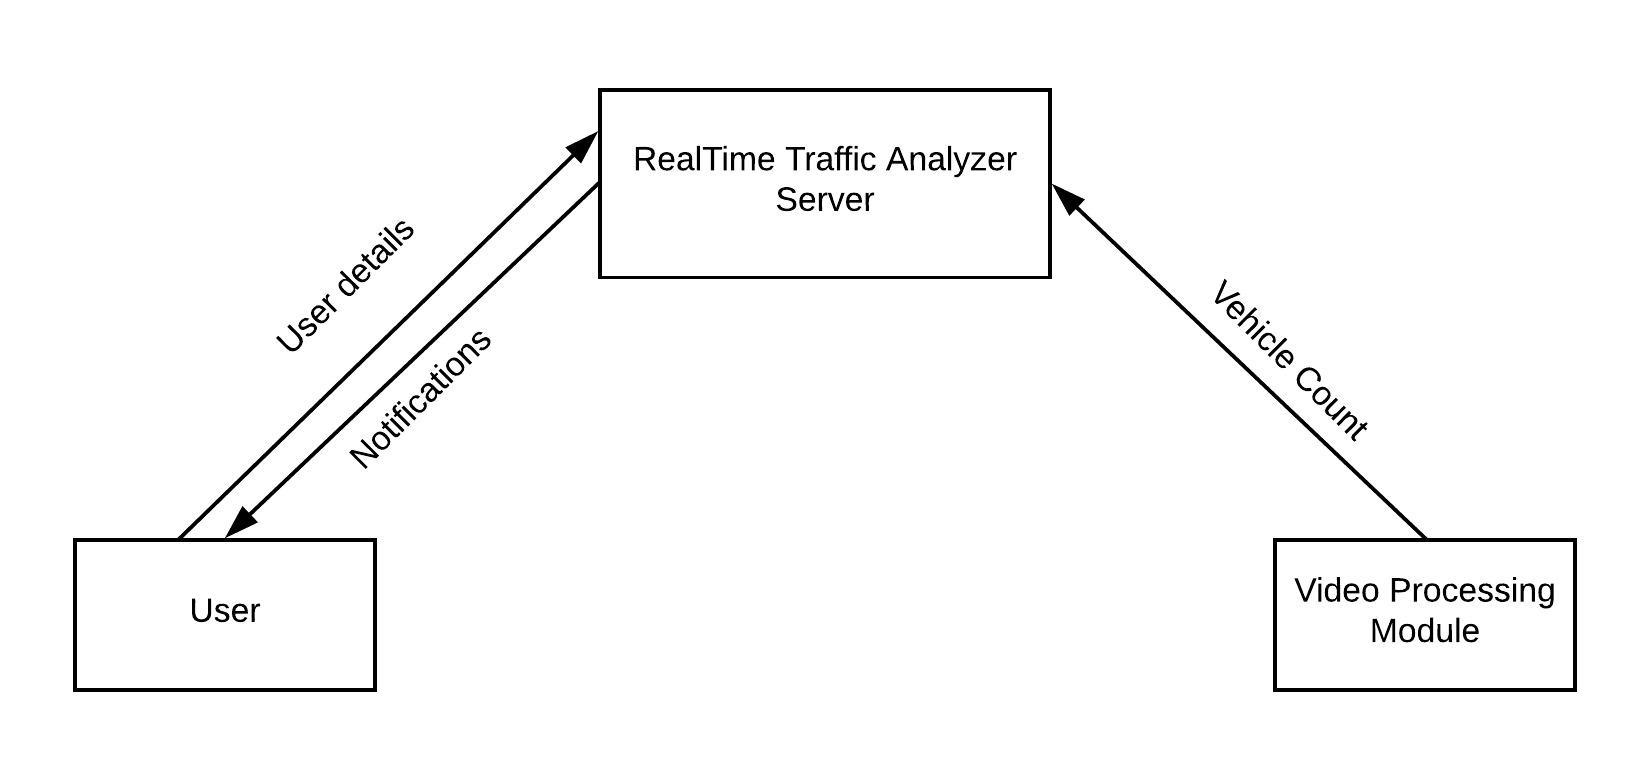
\includegraphics[scale=.8]{arch.png}}\par}
\caption{System Architecture}
\end{figure}\\

\\

The system comprises of three main modules.\\

First module deals with an Android Application where users register with their details, update route details including source, destination, date and time for travel. \\

Second module is an OpenCV application for tracking and detecting vehicles and vehicle count is updated to server in real time. A video sequence of road can be processed and analyzed to detect and count vehicles. Further information, such as the speed of a vehicle or traffic density, can also be calculated by using computer vision. This would directly benefit to two groups of people: road users and traffic administrators. If road users know the real-time traffic information, they can then use the information to choose the best way for traveling and can avoid traffic congestion. On the other hand, traffic administrators can utilize the traffic information in their traffic control systems, resulting to a better traffic management. There are several methods for vehicle detection and counting proposed so far. The real time traffic congestion analyzer for road safety includes, tracking, and counting the vehicles using Blob Detection methods. First, we differentiate the foreground from background in frames by learning the background. Here, foreground detector detects the object and a binary computation is done to define rectangular regions around every detected object. To detect the moving object correctly and to remove the noise some morphological operations have been applied. Then the final counting is done by tracking the detected objects and their regions. Finally, vehicles in a predefined virtual detection zone are recorded and counted.\\

Third module is the server, where all the user and traffic details are stored.The camera footages are processed from client machines located at different locations and traffic details such as average vehicle count per frame in unit time,number off vehicles passed in unit time are periodically sent to the server.  The user logins to server and enter journey details.server periodically keep track of traffic rich locations and notify the active users who travels through those routes

\newpage

\subsection{System Design}
\\
\textbf{Module Description}\\

The proposed system consists of 3 modules: \\ \\
\begin{itemize}
\item ANDROID APPLICATION\\ \\
\begin{figure}[ht] 
{\centering {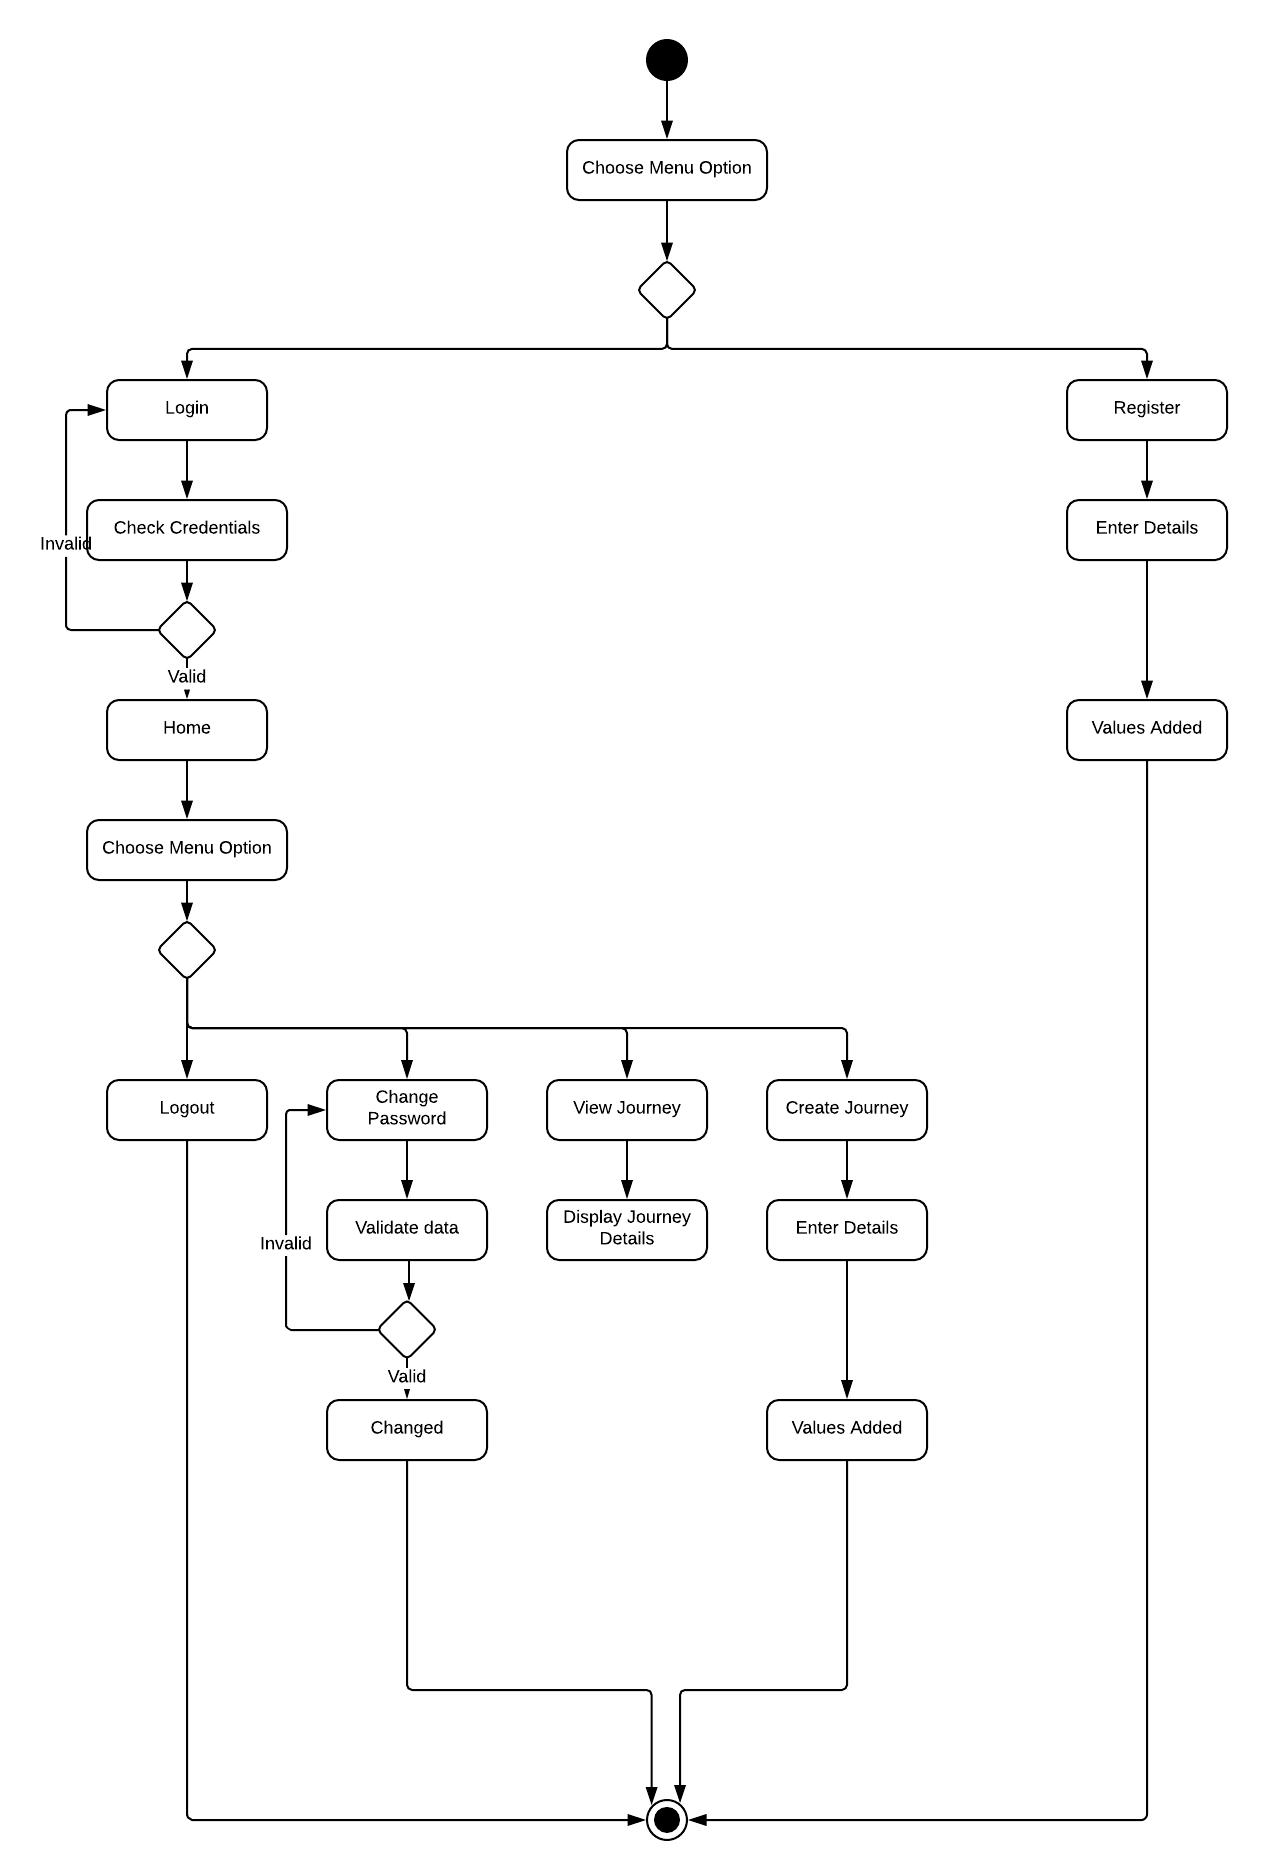
\includegraphics[scale=.59]{uml.png}}\par}
\caption{Activity Diagram}
\end{figure}
\newpage
In order to make the proposed system user friendly, an android application is used to collect the user details. Users can register through the app, can enter details of their journey including source, destination and the route they are going through. From the details stored in the RTA server, they will get an update about the traffic conditions and vehicle count through the android application. The activity diagram is shown above \\ \\
\item VEHICLE DETECTION AND COUNTING\\ \\

\begin{figure}[ht] 
{\centering {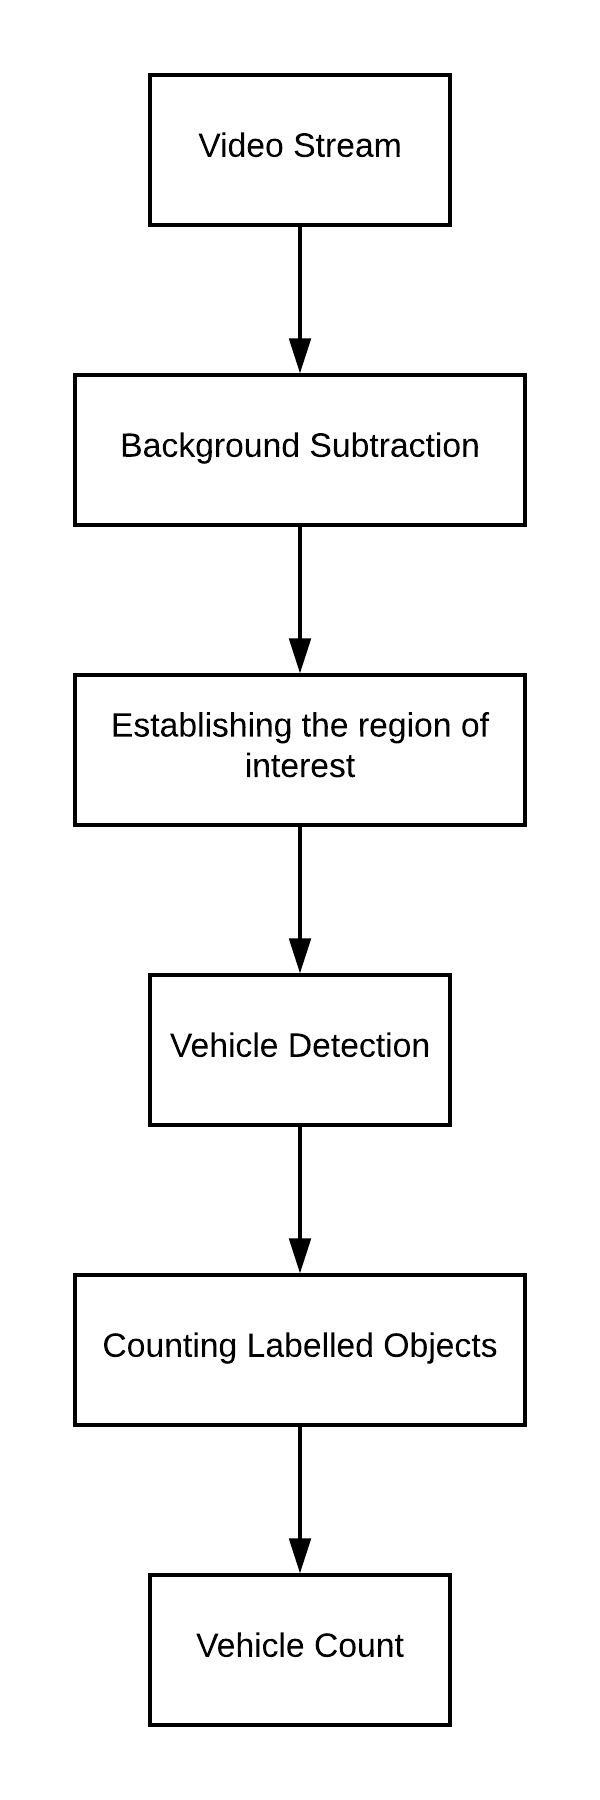
\includegraphics[scale=1]{flow.png}}\par}
\caption{Vehicle Counting Flowchart}
\end{figure}\\ \\

A simple approach was carried out for vehicle detection and counting using Pixel Based Adaptive Segmenter - based object detection, a non-predictive regional tracking and a counting of tracked objects based on simple rules. Pixel-Based Adaptive Segmenter, follows a non-parametric paradigm. Thus, every pixel is modeled by an array of recently observed background values. the decision block decides for or against foreground
based on the current image and a background model. This decision is based on the per-pixel threshold. Moreover, the background model has to be updated overtime in order to allow for gradual background changes.\\
\newpage
This module includes four sub-modules, which is discussed below:


\begin{itemize}
\item BACKGROUND SUBTRACTION\\ \\
Background Subtraction is improved by combining adaptive background generation with two-frame differencing algorithm.  We assume that the video stream is captured with a RGB 24 bits format. We use the luminance component of the RGB image to estimate the motion for each frame. Once we have a robust background model, we can use a method called background subtraction to segment each frame into foreground and background objects.  A pixel would be part of the foreground, when its value is different enough from its corresponding value in the background model. The main difficulty is to evaluate the distance of each pixel in a color frame (in RGB color space) to the corresponding background pixel. This evaluation allows the classification of all the current image pixels in two categories (foreground and background). In some situations, an oversimplification of the method (e.g. a binarization with a static threshold) may cause erroneous segmentation. In most cases, a simple binarization is not sufficient to obtain a clear foreground. We use a morphological closing to fills the missing foreground pixels and a morphological opening to remove the small isolated foreground pixels.\\ \\
\item ESTABLISHING THE REGION OF INTEREST\\ \\
A region of interest (ROI), which will be further processed, as the next step. The user can set the region of interest initially by drawing a line hoizontally or vertically across the video screen. This line seperates the video into two regions, say region A and region B. The vehicle that passes the ROI will be counted and the total count will be passed. \\ \\
\item VEHICLE DETECTION\\ \\
In this step, only pixels in the ROI are considered while the others are deleted. Here, we detect the moving objects using a Background Subtraction (BS) algorithm. For vehicle tracking, we need to use a tracking algorithm called blob tracker algorithm. Then send the foreground mask to cvBlob or OpenCVBlobsLib. The cvBlob library provide some methods to get the centroid, the track and the ID of the moving objects. A bounding rectangle is drawn to track the tracked object and is checked whether this tracked object's centroid passes the ROI. \\ \\
\item VEHICLE COUNTING\\ \\
The main object of this part is to count and register the vehicle flow for each lane. The count of the vehicles that passes the ROI region is the vehicle count and the count of the bounding boxes is the traffic count in that specific area. If there is no vehicle that cross the ROI, it means that vehicle count should be zero. Both the vehicle count and bounding boxes count are updated in the server. \\ \\
\end{itemize}\\ \\
\newpage
\item Real-time Traffic Analyzer SERVER\\ \\
OpenCV application detects and count the vehicles. Counting vehicles gives us the information needed to obtain a basic understanding over the flow of traffic in any region under surveillance. The total count of vehicles, including other traffic details such as source and destination of user are stored on the server. Thus server keeps a track of vehicle count from different locations and checks active users in the route. This will help to make a traffic analysis. The RTA server gets updated on every 15 minutes and notify the user back through the android application.\\ \\
\end{itemize}
\\ \\


\textbf{DataFlow Diagram}\\
 \\ 


A data flow diagram (DFD) is a design tool to represent the flow of data through an informationsystem.A context level DFD can be used to show the interaction between a system and outside entities; it can also show the internal data flows within a system. ram. It often shows the information system as a single circular shape with
no details of its inner workings: what it shows is its relationships with the external entities.A data flow diagram graphically represents: \\ \\ 
\begin{itemize}
\item processes - jobs that are done with the data. A process transforms incoming data flow into outgoing data flow.
\item data stores - files, databases, archives. They can be manual, digital or temporary.
\item external entities - other systems or people beyond the control of the current system.
\item connecting data flows - arrows show how data flows from one place to another.
\end{itemize}


\textbf{Notations in a Data Flow Diagram}\\

\\ \\
\begin{figure}[ht] 
\centering {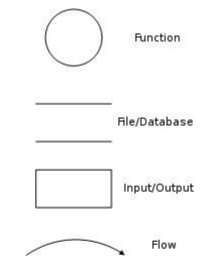
\includegraphics[scale=0.8]{data.png}}
\caption{Notations in dataflow diagram}
\end{figure} \\

\newpage


Context Diagram (Level 0) \\
\begin{figure}[ht]
{\centering {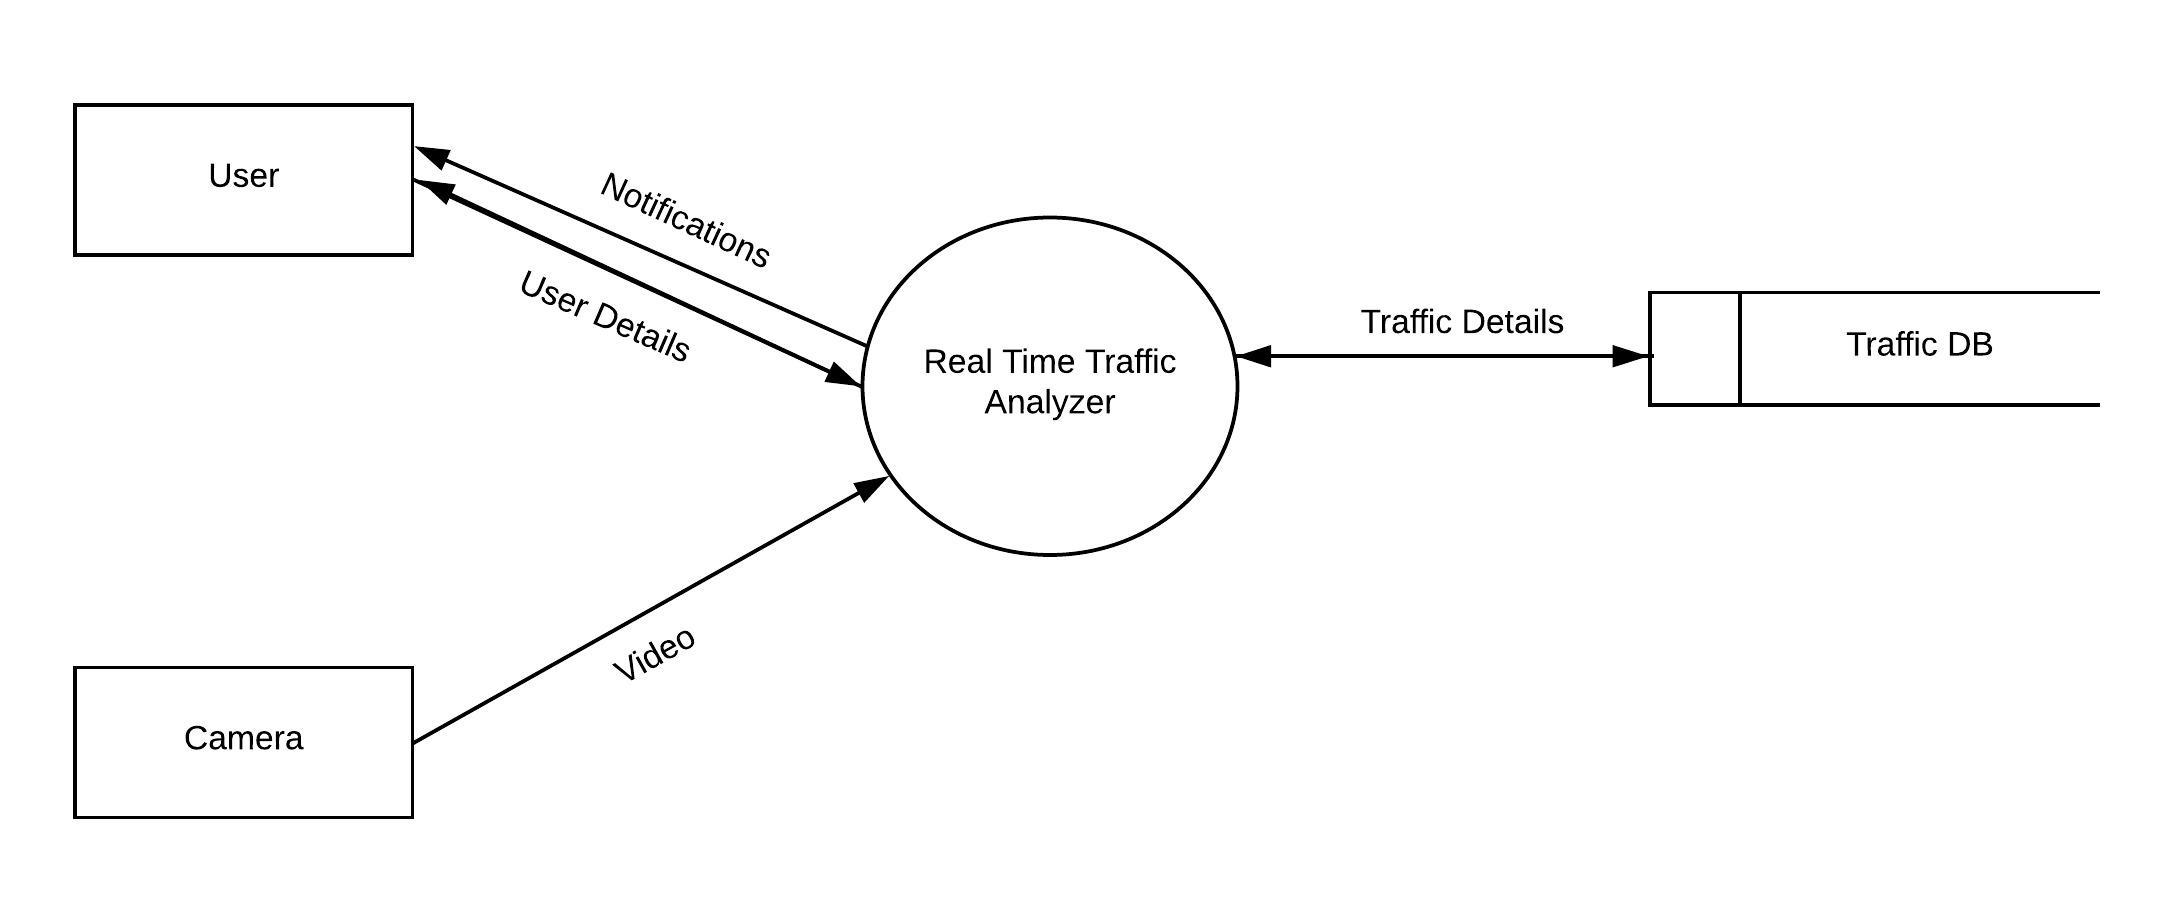
\includegraphics[scale=0.75]{l0.png}\par}} 
\caption{Level 0 DFD}
\end{figure}\\



Top Level DFD(Level 1)\\
\\
\begin{figure}[ht]
{\centering {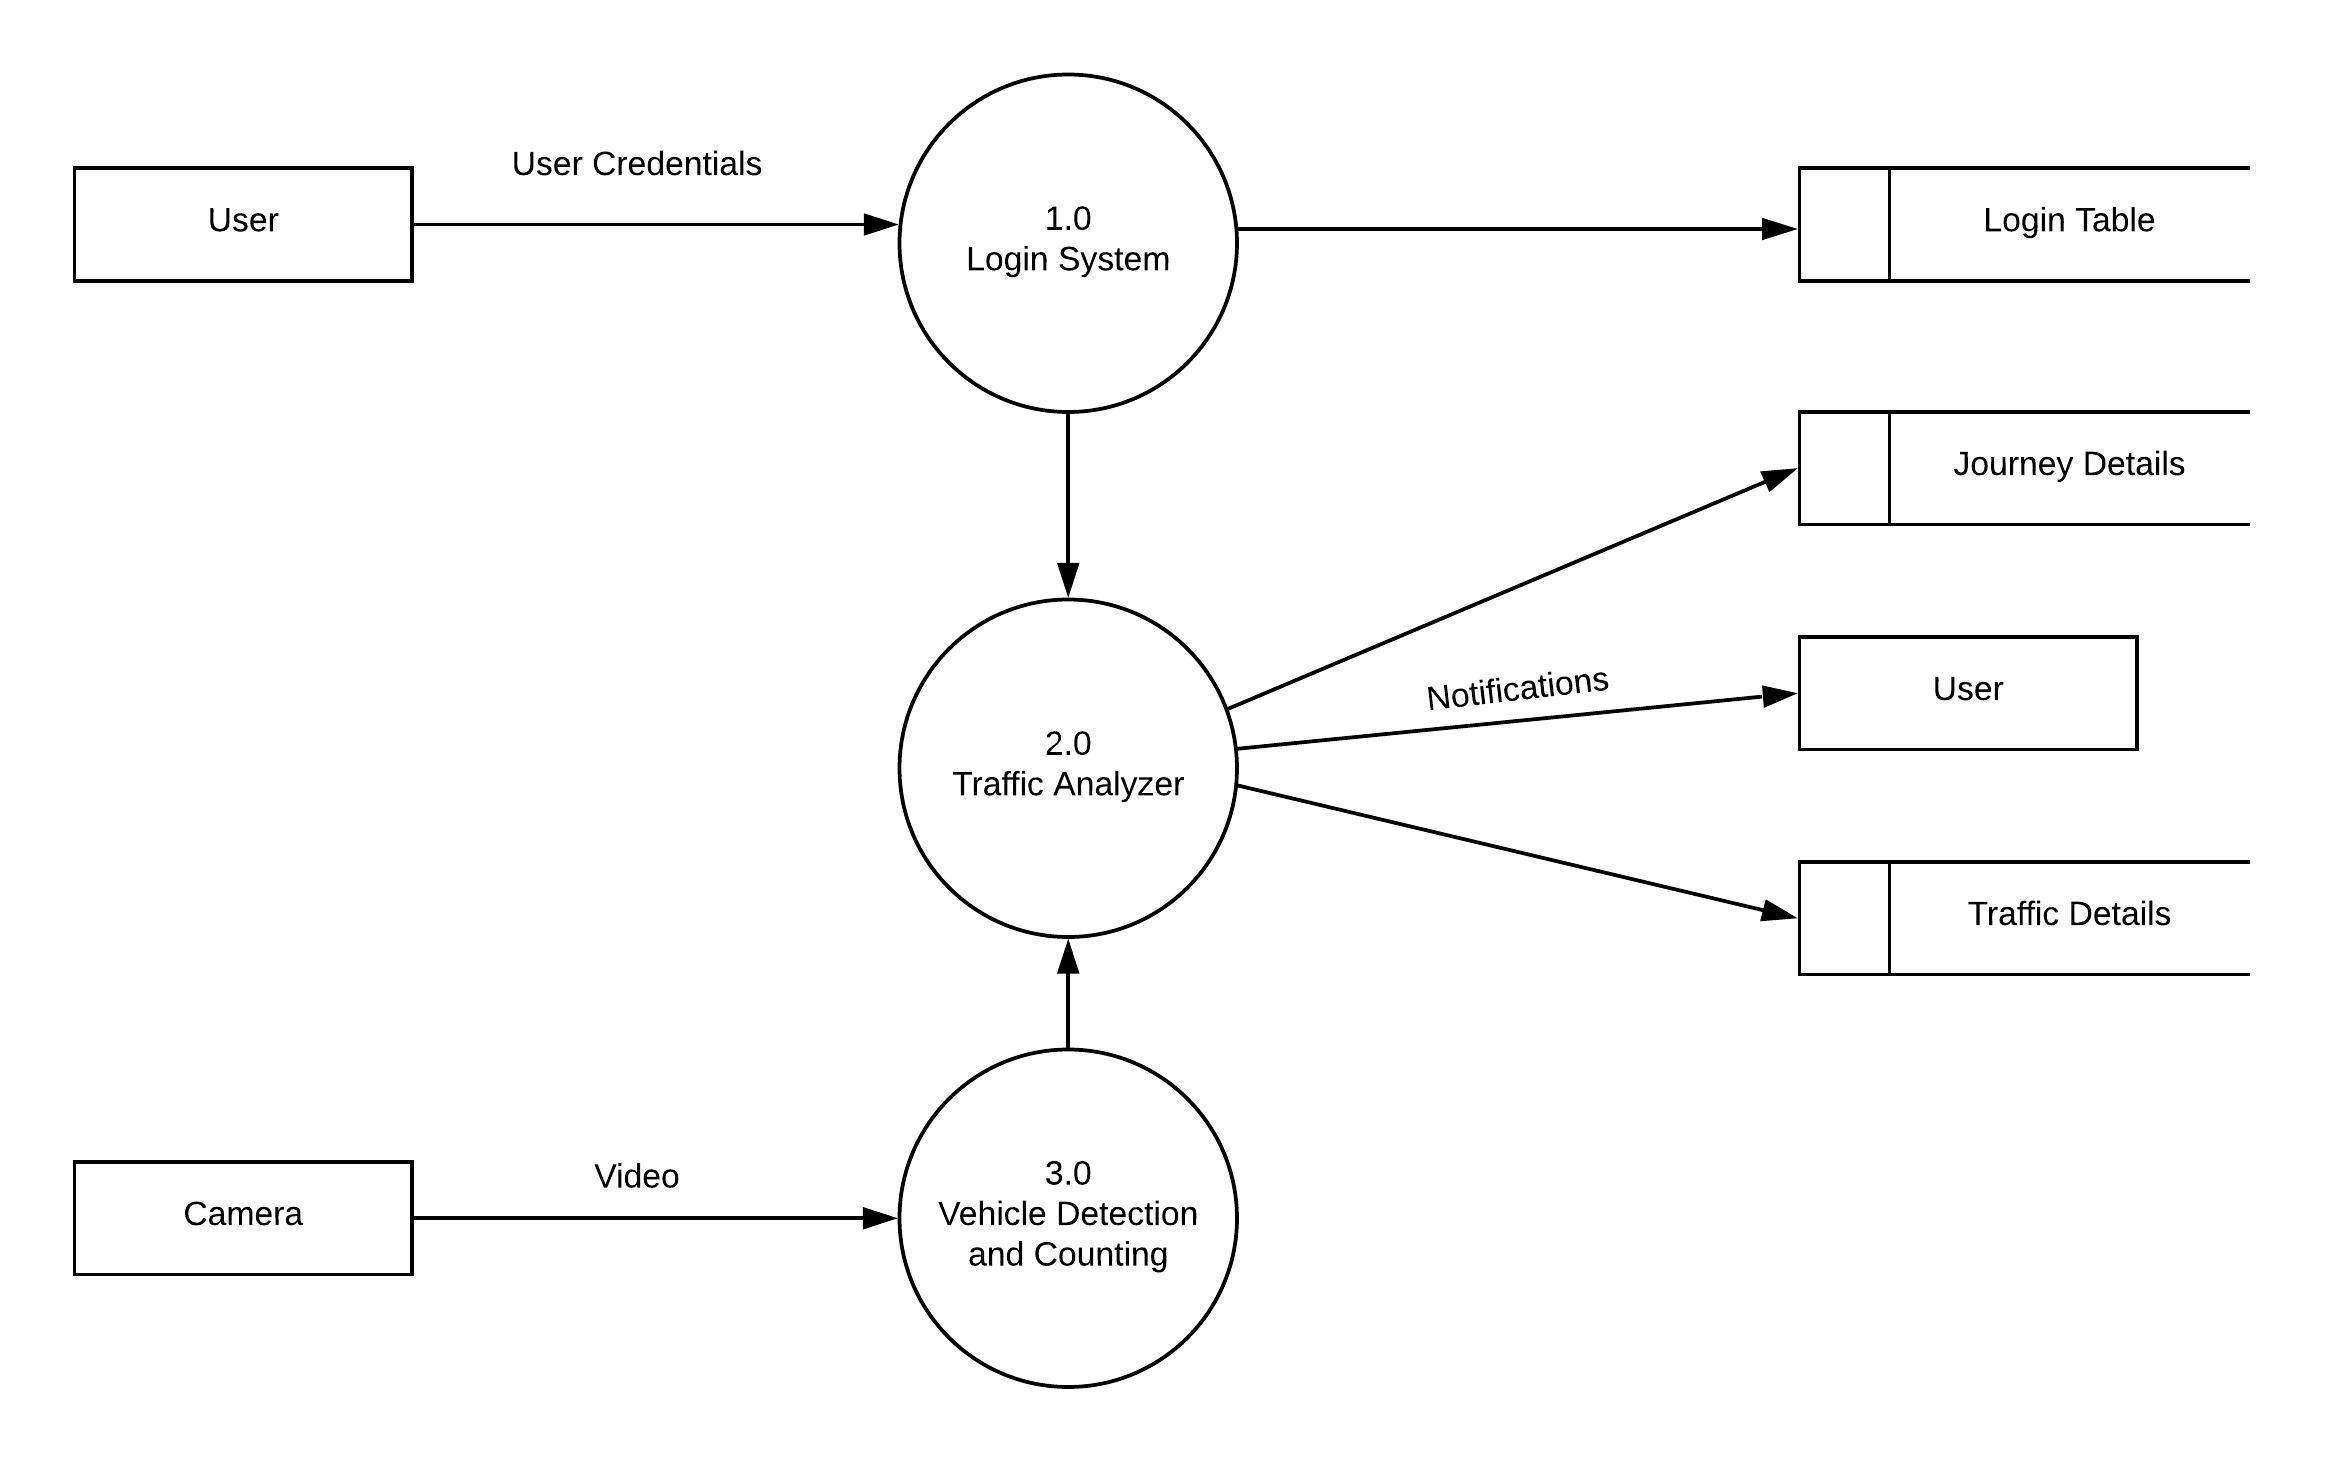
\includegraphics[scale=0.75]{l1.png}\par}}
\caption{Level 1 DFD}
\end{figure}

\newpage

Level 2\\
\begin{figure}[ht]
{\centering {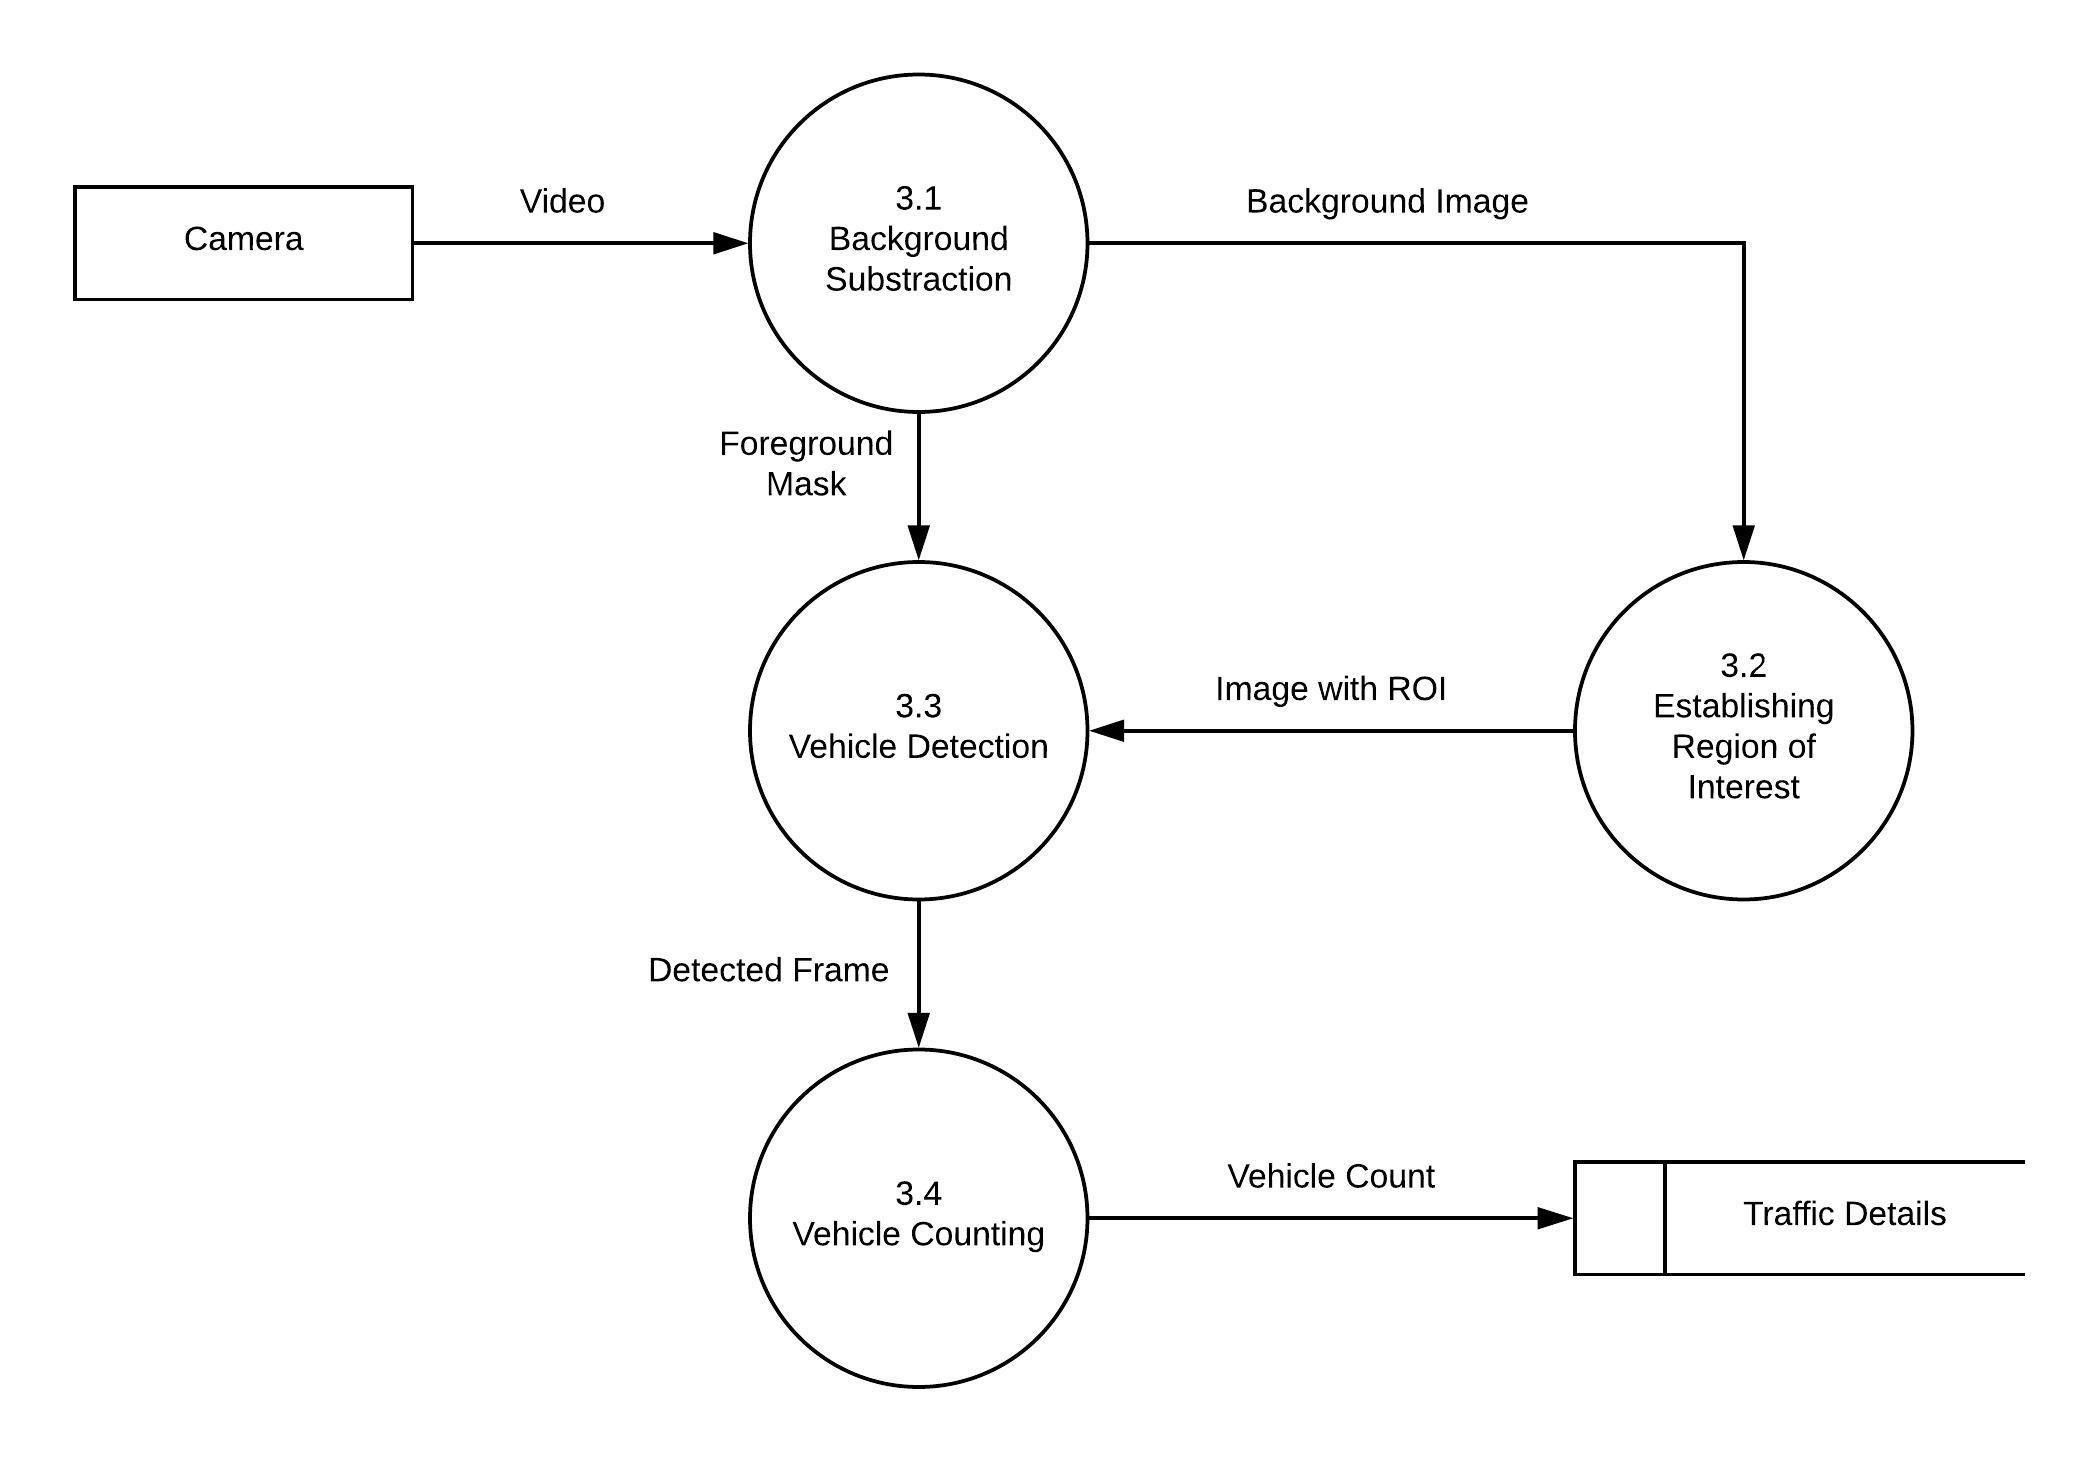
\includegraphics[scale=0.75]{l2.png}\par}}\\
\caption{Level 2 DFD }
\end{figure}\\

Level 3\\
\begin{figure}[ht]
{\centering {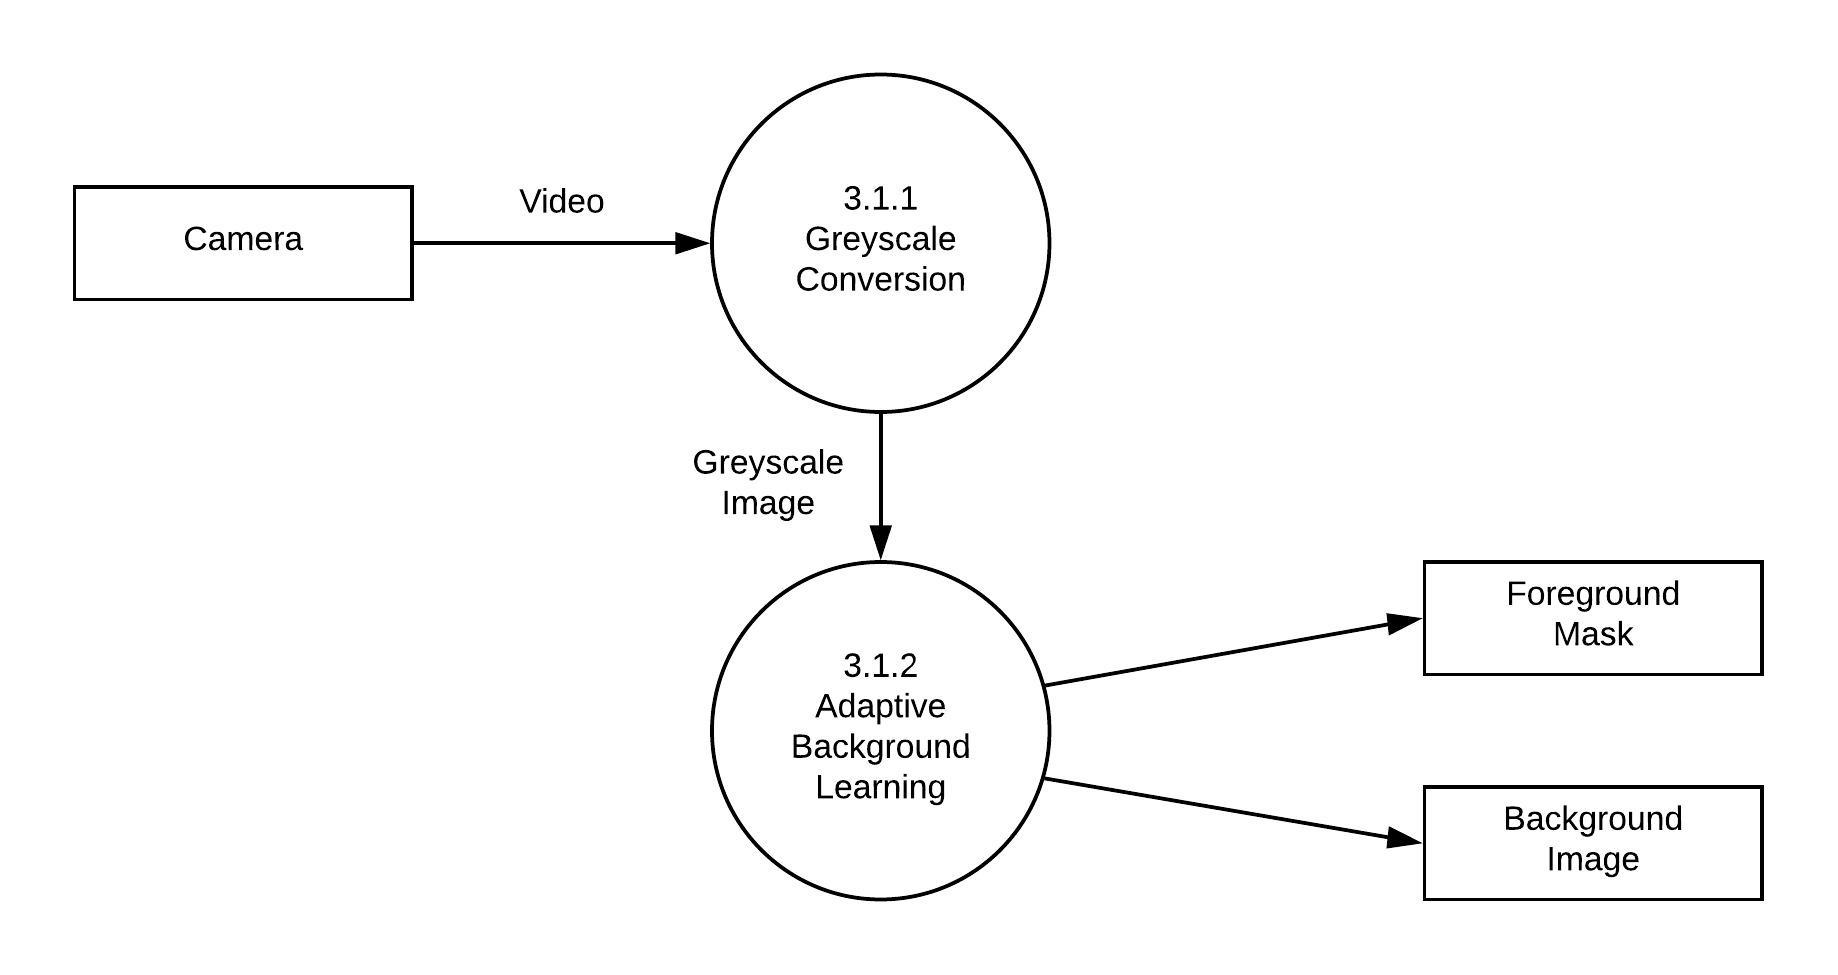
\includegraphics[scale=0.75]{l3.png}\par}}\\
\caption{Level 3 DFD}
\end{figure}\\

\newpage
\subsection{Database Design}

Table name: login\\
Description: Login details\\
Constraints: uname (primary key)\\
\\
\begin{table}[ht]
\begin{tabular}{|c|c|c|} 
\hline
Field  & Data type & Description \\  
\hline
uname& varchar(10)& username \\ 
\hline
password &  varchar(20) & password \\
\hline
usertype &  varchar(10) & type of the user \\
\hline
\end{tabular}
\caption{Login Details }
\end{table}


Table name: route\\
Description: Route Details\\
Constraints: routeid (primary key)\\
\\
\begin{table}[ht]
\begin{tabular}{|c|c|c|} 
\hline
Field  & Data type & Description \\  
\hline
routeid& int(5)& Route id \\ 
\hline
routename&  varchar(20) & Route name \\
\hline
maxvcount&  int(5) & vehicle count \\
\hline
\end{tabular}
\caption{Route Details }
\end{table}

Table name: users\\
Description: User details\\
Constraints: id (primary key)\\
\\
\begin{table}[ht]
\begin{tabular}{|c|c|c|} 
\hline
Field  & Data type & Description \\  
\hline
id& int(20)& user id \\ 
\hline
username&  varchar(70) & username \\
\hline
password&  varchar(40) & password \\
\hline
email &  varchar(50) & email id \\
\hline
createdat &  datetime & registered time \\
\hline
updatedat &  datetime & updated time \\
\hline
name &  varchar(50) & name of the user \\
\hline
mobile &  bigint(10) & mobile no \\
\hline
status &  varchar(10) & status of the user \\
\hline
\end{tabular}
\caption{User Details }
\end{table}


Table name: journeydetails\\
Description: Journey details\\
Constraints: id (primary key)\\
\\
\begin{table}[ht]
\begin{tabular}{|c|c|c|} 
\hline
Field  & Data type & Description \\  
\hline
id& int(20)& id number \\ 
\hline
userid &  int(20) & userid, Foreign key \\
\hline
sdate&  date & start date \\
\hline
stime &  time(50) & start time \\
\hline
routeid &  int(5) & routeid, Foreign key \\
\hline
source &  varchar(20) & Source \\
\hline
destination &  varchar(20) & destination \\
\hline
duration &  tinyint(4) & duration of the journey \\
\hline
\end{tabular}
\caption{Journey Details }
\end{table}


Table name: activejourney\\
Description: Active Journey details\\
Constraints: id (primary key)\\
\\
\begin{table}[ht]
\begin{tabular}{|c|c|c|} 
\hline
Field  & Data type & Description \\  
\hline
id & int(5)& Active Journey id \\ 
\hline
routeid &  int(5) & Route id, Foreign key \\
\hline
date&  date & Journey Date \\
\hline
roicount&  int(5) & Traffic count \\
\hline
avgcount&  int(5) & Total vehicles count \\
\hline
\end{tabular}
\caption{Active Journey Details}
\end{table}

\newpage
\subsection{User Interface Design}
\\
\begin{figure}[ht]
{\centering {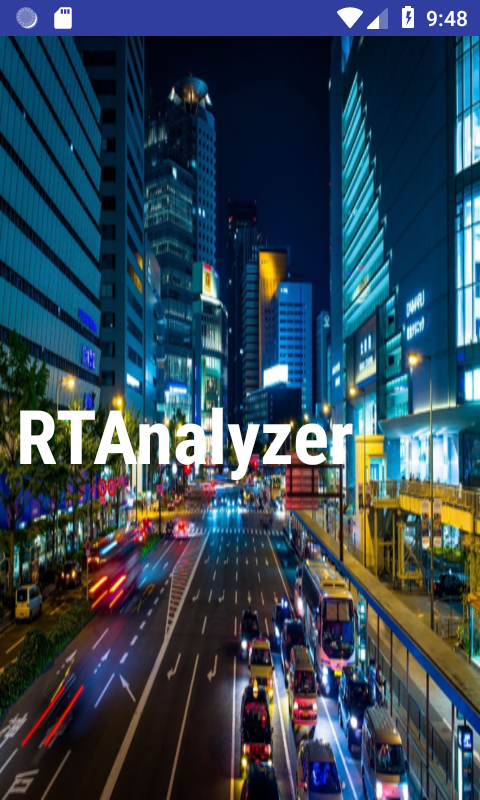
\includegraphics[scale=0.35]{splash.png}\par}}\\
\caption{Splash screen for Android Application}
\end{figure}\\



\\
\begin{figure}[ht]
{\centering {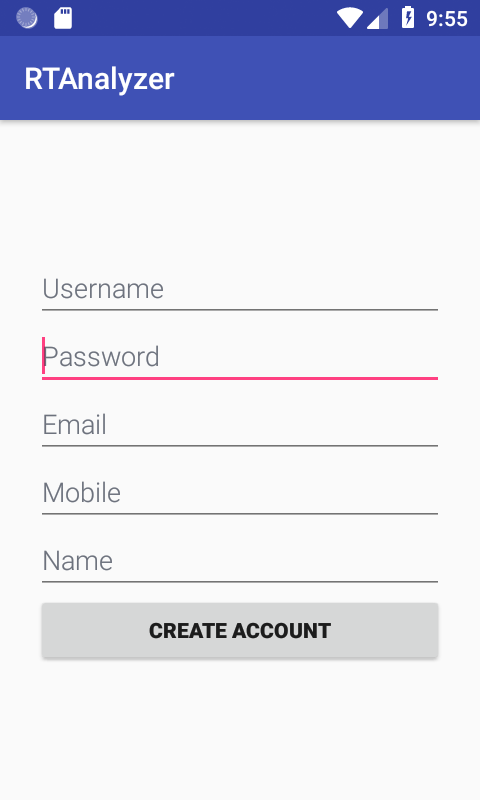
\includegraphics[scale=0.35]{register.png}\par}}\\
\caption{User Registration}
\end{figure}\\


\\
\begin{figure}[ht]
{\centering {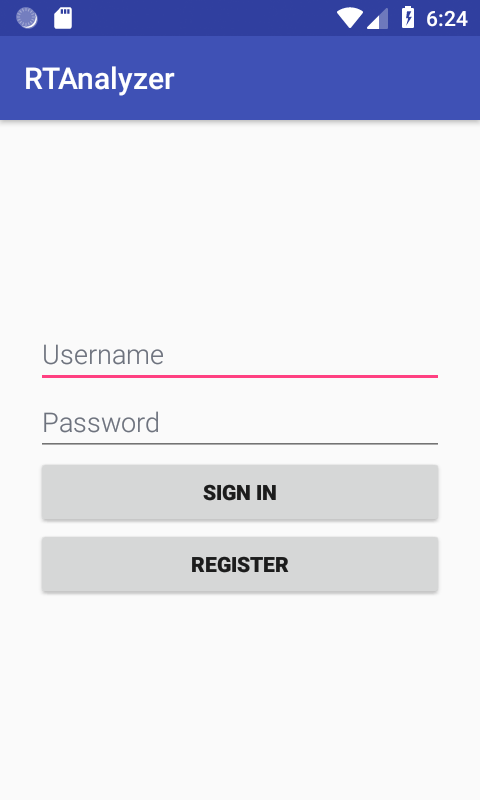
\includegraphics[scale=0.35]{login.png}\par}}\\
\caption{Login page}
\end{figure}\\

\newpage

\\
\begin{figure}[ht]
{\centering {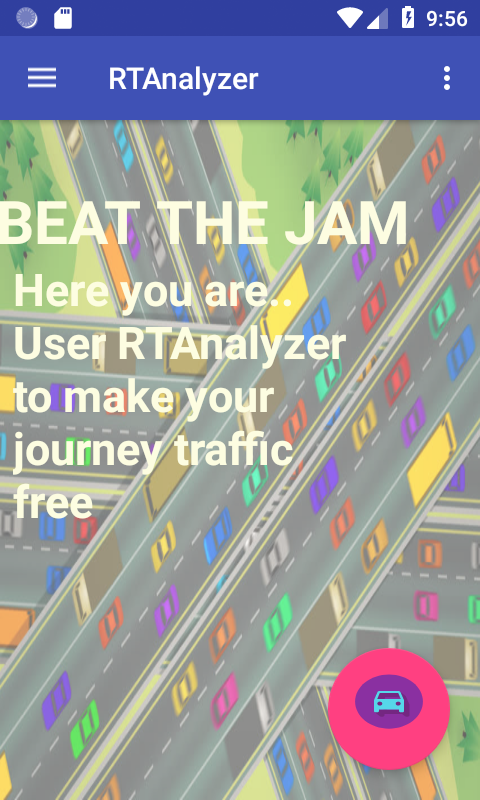
\includegraphics[scale=0.35]{home.png}\par}}\\
\caption{Home page}
\end{figure}\\

\newpage

\\
\begin{figure}[ht]
{\centering {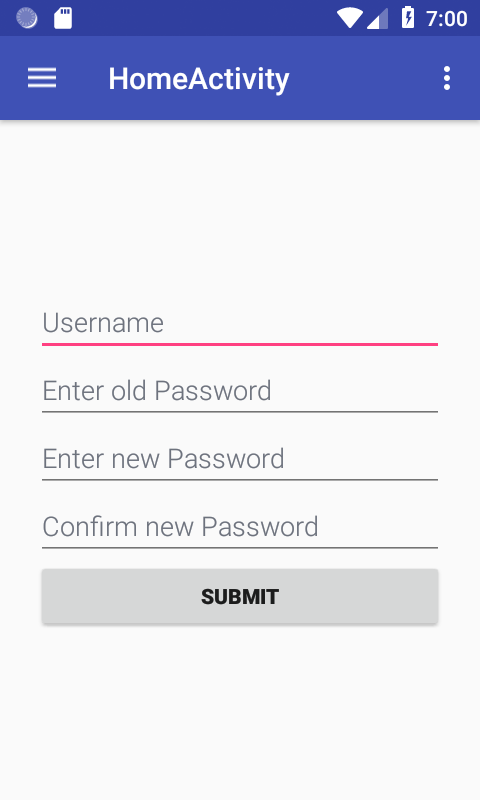
\includegraphics[scale=0.35]{chpwd.png}\par}}\\
\caption{Change Password page}
\end{figure}\\


\\
\begin{figure}[ht]
{\centering {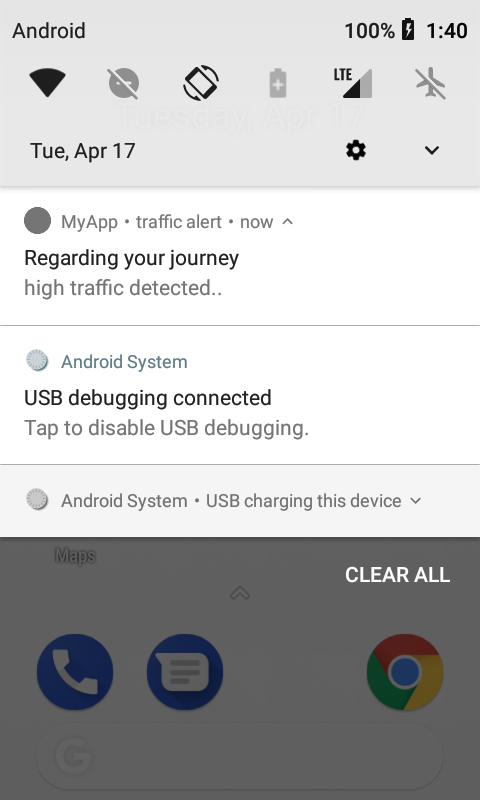
\includegraphics[scale=0.35]{notification.png}\par}}\\
\caption{Notification}
\end{figure}\\


\\
\begin{figure}[ht]
{\centering {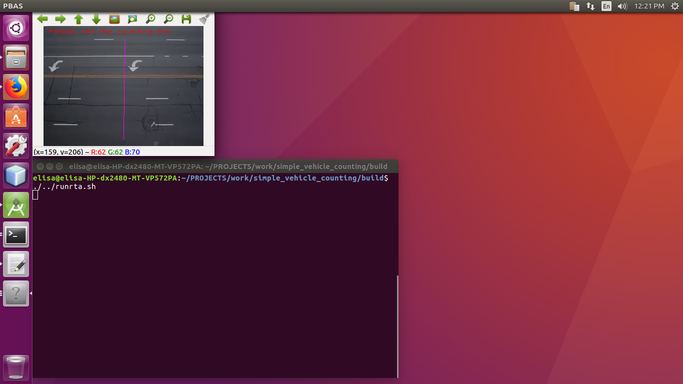
\includegraphics[scale=0.50]{roi.png}\par}}\\
\caption{Setting Region of Interest}
\end{figure}\\



\\
\begin{figure}[ht]
{\centering {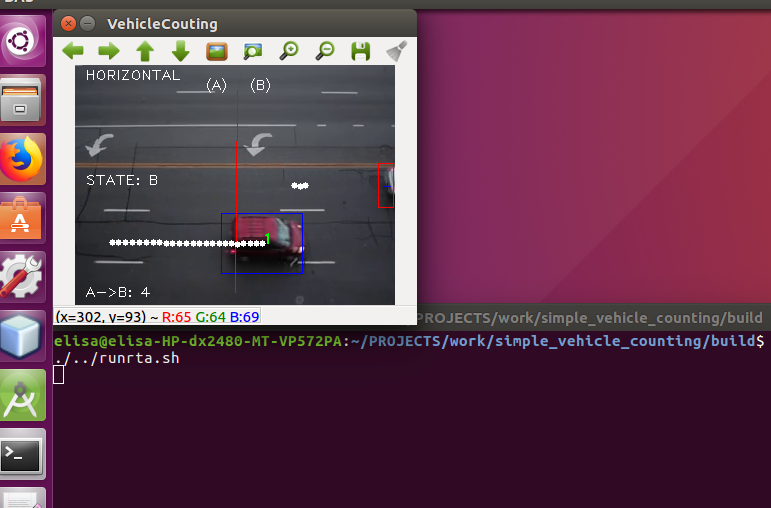
\includegraphics[scale=0.50]{counting.png}\par}}\\
\caption{Vehicle Counting}
\end{figure}\\[1 cm]




\\
\begin{figure}[ht]
{\centering {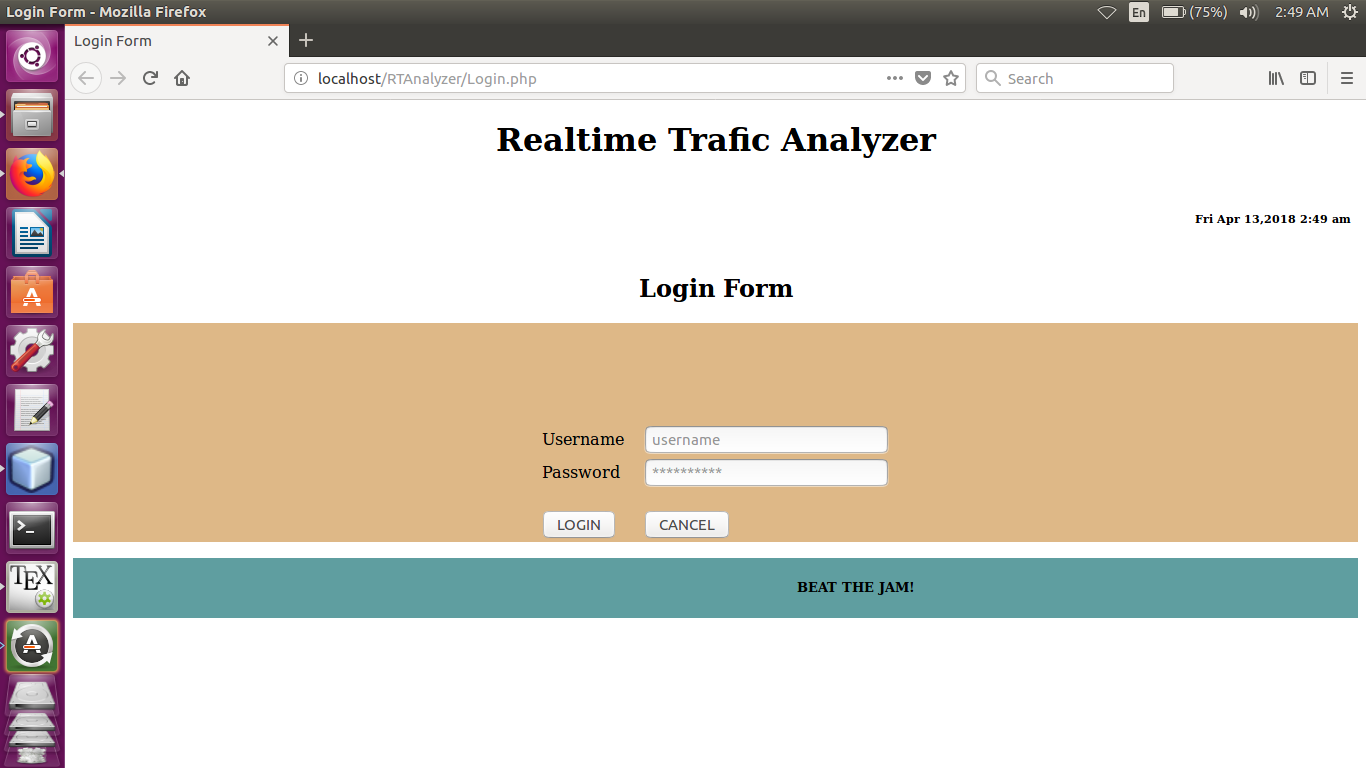
\includegraphics[scale=0.30]{sl.png}\par}}\\
\caption{Login Page of server}
\end{figure}\\



\\
\begin{figure}[ht]
{\centering {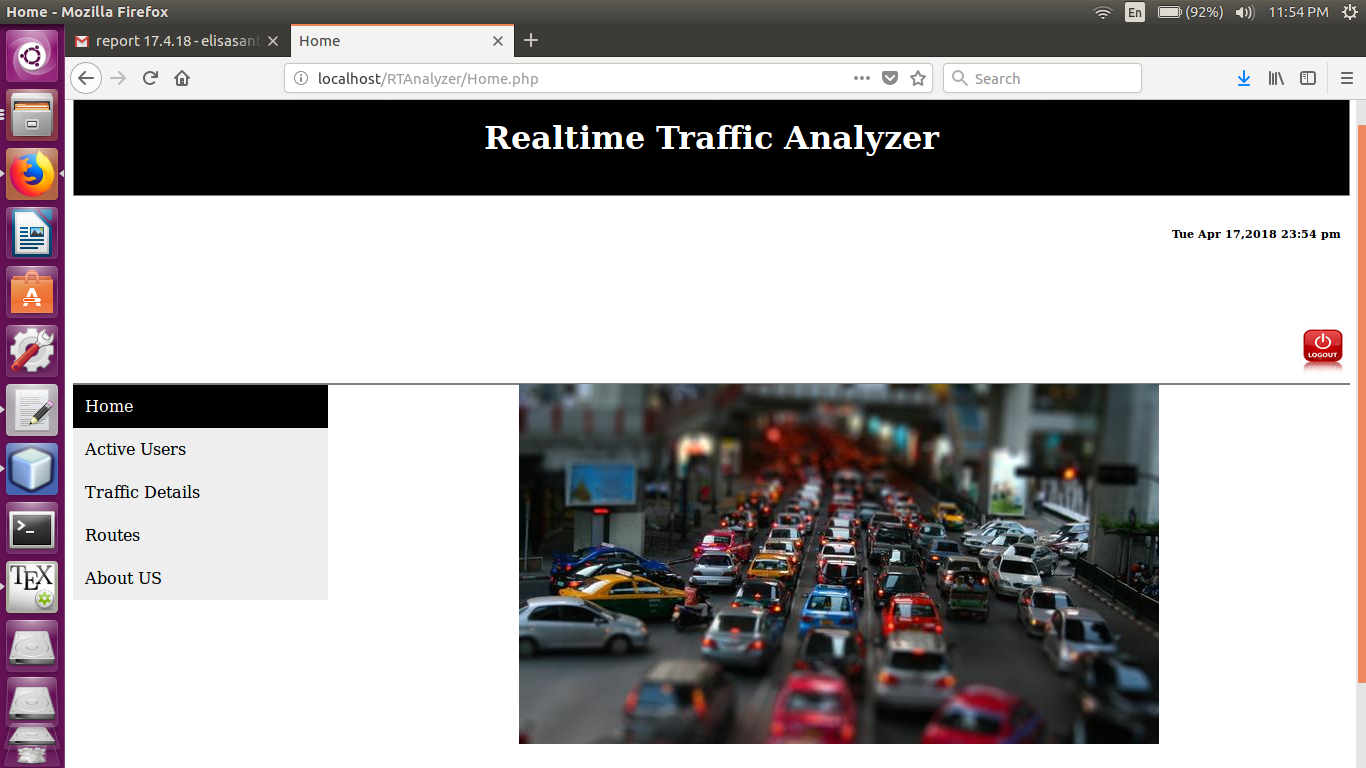
\includegraphics[scale=0.30]{sh.png}\par}}\\
\caption{Home page of server}
\end{figure}\\



\\
\begin{figure}[ht]
{\centering {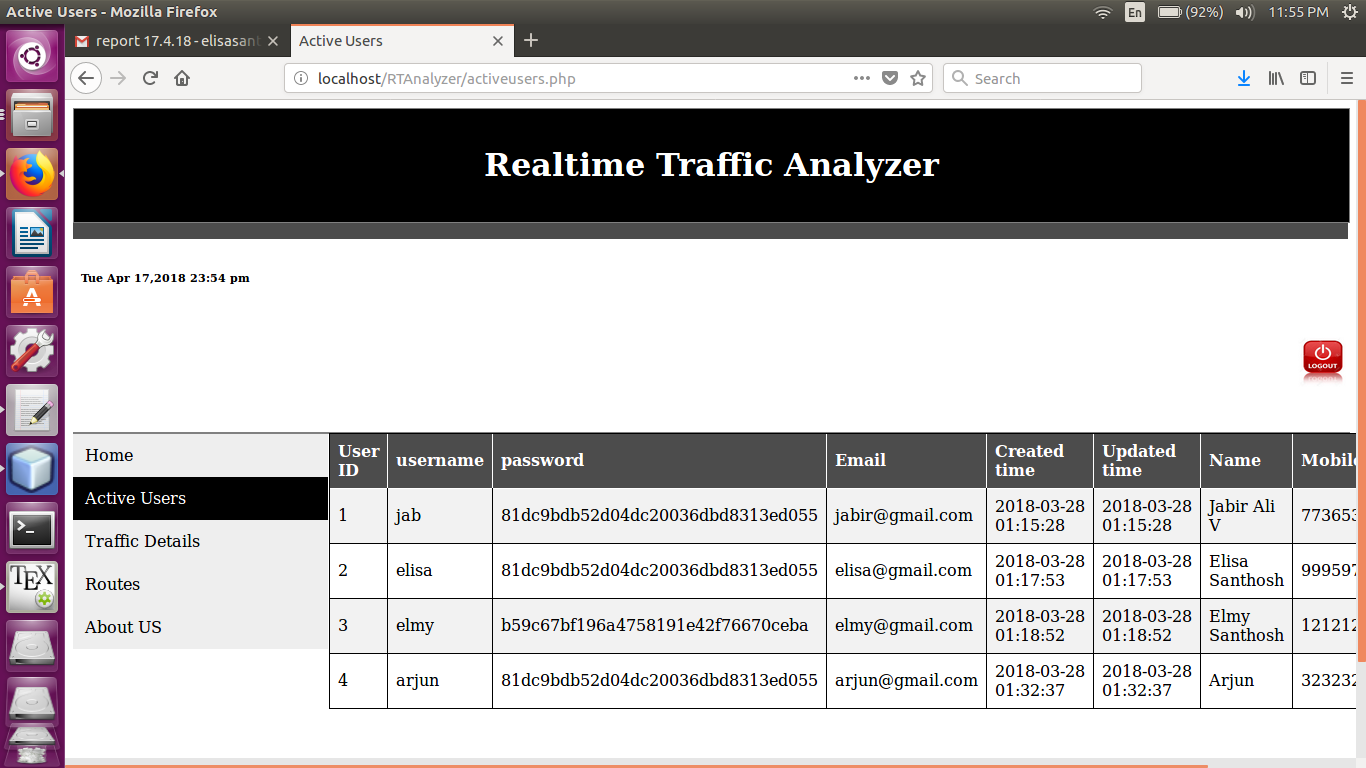
\includegraphics[scale=0.30]{sau.png}\par}}\\
\caption{Active Users}
\end{figure}\\



\\
\begin{figure}[ht]
{\centering {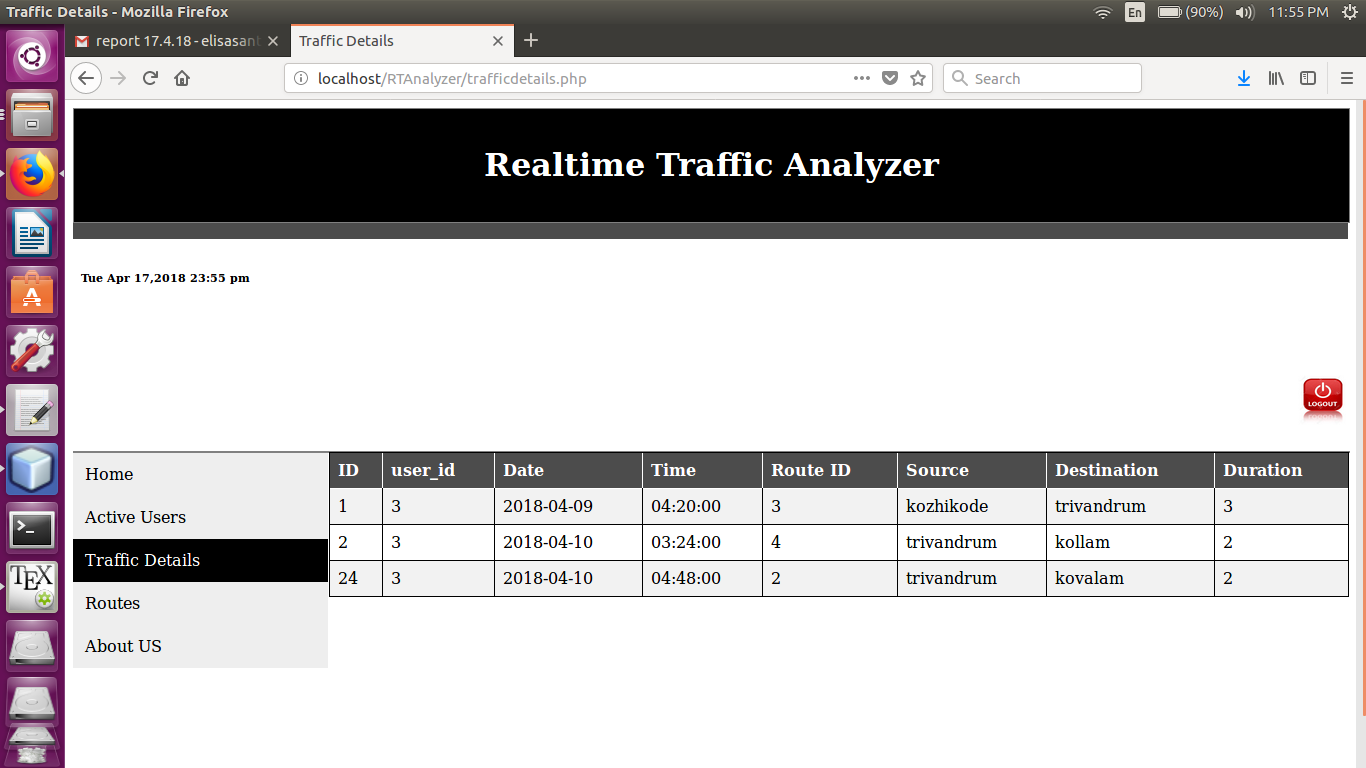
\includegraphics[scale=0.30]{std.png}\par}}\\
\caption{Traffic Details}
\end{figure}\\



\\
\begin{figure}[ht]
{\centering {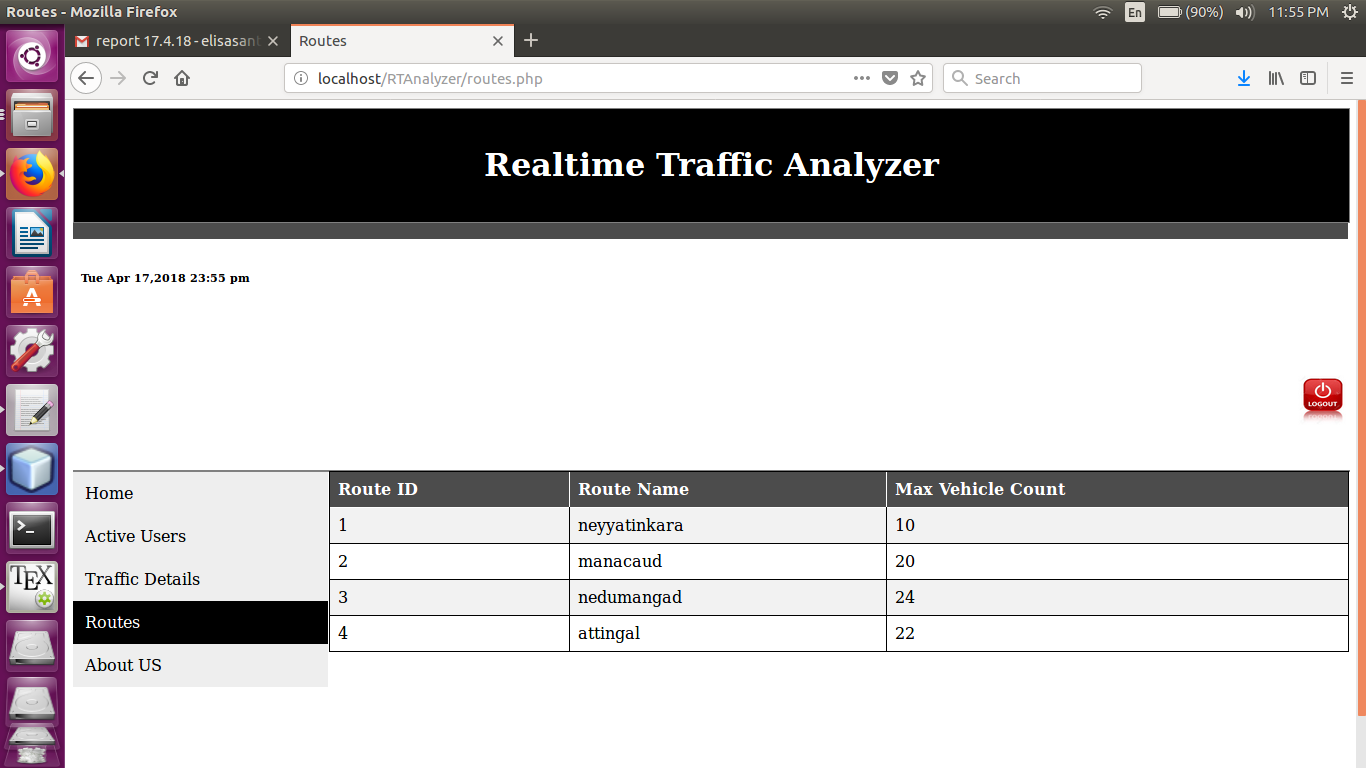
\includegraphics[scale=0.30]{sr.png}\par}}\\
\caption{Route Details}
\end{figure}\\



\\
\begin{figure}[ht]
{\centering {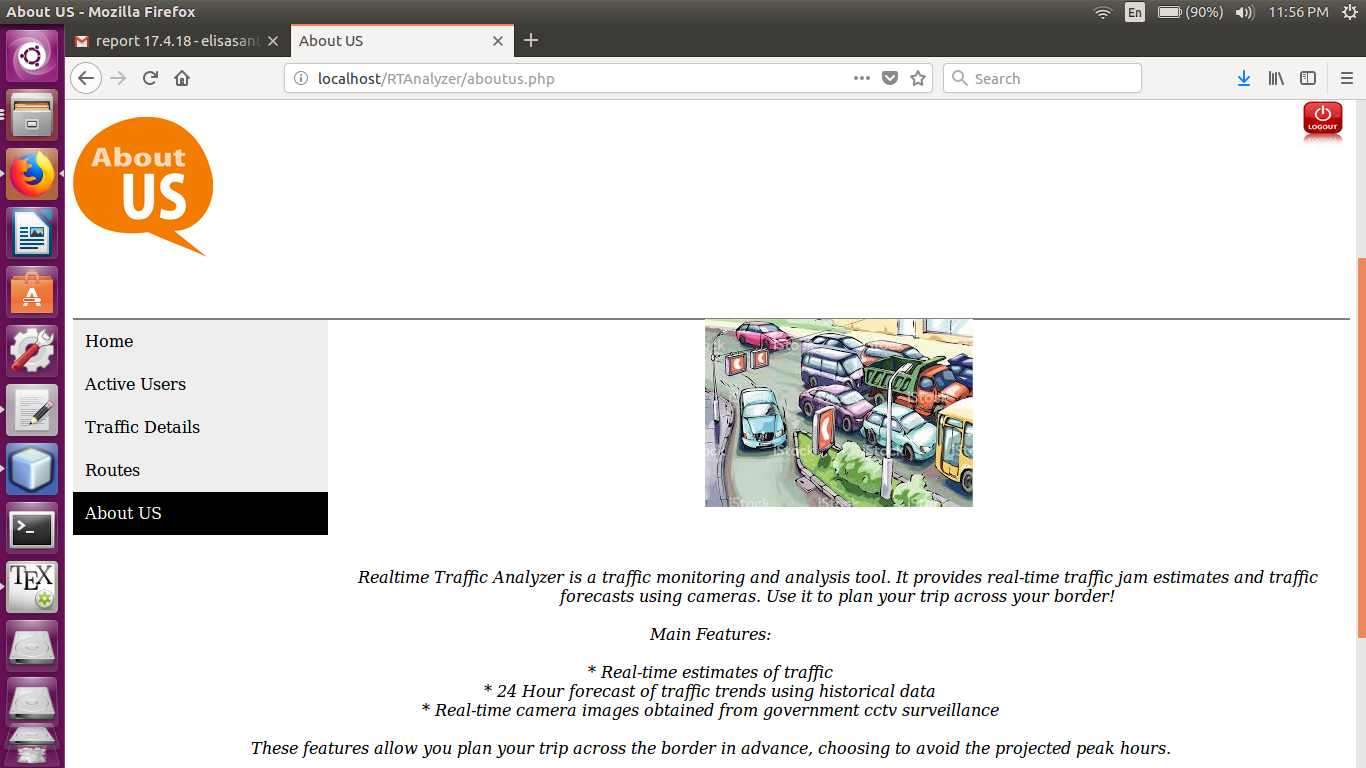
\includegraphics[scale=0.30]{abt.png}\par}}\\
\caption{Server About US}
\end{figure}\\[1 cm]